\documentclass[output=paper]{LSP/langsci} 

\title{Statistical MWE-aware parsing} 

\author{\texorpdfstring{
Mathieu Constant\affiliation{ATILF UMR 7118, Universit\'e de Lorraine/CNRS}\and 
Gülşen Eryiğit\affiliation{Istanbul Technical University}\and 
Carlos Ramisch\affiliation{Aix-Marseille Universit\'e}\and
Mike Rosner\affiliation{University of Malta}\lastand
Gerold Schneider\affiliation{University of Konstanz and University of Zurich}}{Mathieu Constant, Gülşen Eryiğit, Carlos Ramisch, Mike Rosner, Gerold Schneider}
}

\lehead{M. Constant, G. Eryi{\v{g}}it, C. Ramisch, M. Rosner \& G. Schneider}
%\shorttitlerunninghead{}

% \chapterDOI{} %will be filled in at production
% \epigram{}


\abstract{
This chapter aims at presenting different strategies that have been designed to incorporate multiword expression (MWE) identification in the process of syntactic parsing using statistical approaches. We discuss MWE representation in treebanks, pipeline and joint orchestrations, the integration of external lexicons and the evaluation of MWE-aware parsers, concluding with our suggestions for future research.% Volume: 10-15 pages
}

\begin{document}
\maketitle

%\input{constantetal/01-intro}
\section{Introduction}

Supervised \main{statistical parsing} is nowadays an important and challenging field of \main{natural language processing (NLP)}. 
It consists in predicting the most probable syntactic structure of a new sentence, given a statistical model that has been trained on a \main{treebank}, that is, a syntactically annotated corpus.
Since the seminal works of \citet{nivre04b} for dependency parsing and \citet{arun05} for constituency parsing, a new research line has emerged: incorporating the analysis of \main{multiword expressions (MWEs)} in such parsers.
The main objective of this chapter is to present different approaches that have been developed and evaluated for statistical MWE-aware parsing systems. 


The design of MWE-aware parsers must address the following questions:
How are MWEs represented in combination with syntactic trees? 
When is MWE identification performed with respect to parsing? 
What algorithms and machine learning techniques are to be used for the two tasks? 
How can external lexical resources be integrated to improve MWE coverage? 
How are systems evaluated?


Answering the question about MWE \main{representation} is fundamental as it enables the definition of a system's output. Hence, it influences the design of datasets used for training and test, including treebanks, as shown in Section~\ref{sec:representation}.

% \item 
The \main{orchestration} issue is also crucial in order to position MWE identification with respect to parsing: should it be performed before, during or after it? The answer is not straightforward as it might depend on the type of MWE \citep{eryigit:2011:mes:2206359.2206365}. Orchestration also implies determining how the two components interact. 
For instance, in pipeline strategies (before or after) discussed in Section~\ref{sec:pipeline}, should the intermediate input/output be computed using MWE concatenation strategies or MWE substitution ones? 
Joint strategies (during)  discussed in Section~\ref{sec:joint} alongside n-best strategies, might involve different methods like adapting a grammatical formalism for constituent parsing \citep{green13} or concatenating arc labels in dependency parsing \citep{vincze13}.
% \item 

Concerning \main{algorithms} and machine learning, most techniques use worka\-round approaches by adapting the MWE-aware representation to existing representations directly exploitable by off-the-shelf tools \citep{nasretal15}. Nonetheless, new parsing algorithms have been recently proposed that include specific handling of MWEs, notably when using joint strategies \citep{nivre:2014}. 
% \item 

The integration of \main{exogenous lexical knowledge} in the system, discussed in  Section~\ref{sec:resources}, is non-trivial but potentially helpful. Indeed, supervised systems are trained on datasets of limited size. Therefore, one drawback of such systems is the limited coverage in terms of MWEs. One possible solution consists in integrating knowledge coming from large-scale MWE lexicons, either manually built and/or validated \citep{candito2014strategies} or automatically acquired \citep{schneider:2012}.

% \item 
The last issue concerns \main{evaluation}: what is the impact of MWE identification on syntactic parsing and vice-versa? What types of measure are adequate to quantify this impact? We try to answer these questions in Section~\ref{sec:evaluation}.
% \end{enumerate}


The outline of this chapter is as follows. First, we briefly explain some basic concepts and terms in statistical parsing in Section~\ref{sec:parsing}. Then, each section addresses the questions above. We conclude in Section~\ref{sec:conclusions} by providing a summary of the current research in statistical MWE-aware parsing and presenting pointers that, in our opinion, may lead to significant advances in the field in the future.



%\input{constantetal/02-statisticalparsing}
\section{Statistical parsing}
\label{sec:parsing}

Parsing, also referred as syntactic analysis, is the process of assigning a syntactic structure to a given input sentence.
The analysis is aimed at producing a valid syntactic tree conforming to a hand-written or automatically induced language grammar.
With the emergence of manually annotated datasets (i.e. treebanks) and machine learning techniques,
statistical parsing \citep{collins1996new,charniak2000maximum} has become the dominant approach in the parsing literature. 

Statistical parsing aims at selecting the most probable parse tree from the set of all possible parse trees for a given sentence. 
These data-driven parsing models may be basically grouped under generative or discriminative approaches.
\main{Generative} parsing models generally rely on a grammatical formalism whereas \main{discriminative} ones are usually performed without any underlying grammar.
There exist also joint approaches where a discriminative model is used to rerank the top n candidates of a generative parser.

Constituency and dependency formalisms are the most two common parsing formalisms used in statistical parsing.
Figure~\ref{fig:wws} and Figure~\ref{fig:flat} each provide constituency and dependency parse tree samples
for the sentence \expl{The prime minister made a few good decisions.} 

In the \main{constituency formalism}, a sentence is regarded as being composed of phrases and parsing is the task of determining the underlying \emph{phrase structure}.
For example, a statistical generative constituency parser aims to assign probabilities to a parse tree by combining the probabilities of each of its sub-phrases.
In the \main{dependency formalism}, parsing is defined as correctly determining the dependency relations between words of an input sentence. More precisely,
the aim of dependency parsing is to correctly determine the dependent-head relationships between words and also the type of these relationships such as subject, object, predicate.
Dependency parsing is nowadays strikingly more popular than constituency parsing and attracts the attention of an ever-growing community in NLP.
Furthermore, most existing MWE-aware parsers are developed in the dependency framework.
Therefore, in this chapter, we focus mainly on different orchestration scenarios applied for different \emph{statistical dependency parsing} approaches.


The two commonly used approaches for statistical dependency parsing in the literature are transition based \citep{yamada2003statistical,nivre2007maltparser} and graph-based \citep{eisner1996three,mcdonald-lerman-pereira:2006:conll-x,nakagawa:2007:emnlp-conll2007}. 
\main{Transition-based} approaches treat the dependency parsing task as the determination of parsing actions (such as push/pop operations in a shift-reduce parser) by the use of a machine learning classifier. \main{Graph-based} approaches treat parsing as finding the most likely path within a graph, such as the highest-scoring directed spanning tree in a complete graph. Most MWE-aware parsing strategies are adaptations of standard parsers experimenting with various models of orchestration concerning the scheduling of MWE identification with respect to syntactic analysis.

MWEs pose \main{challenges} for all areas of NLP, and statistical parsing is not an exception.
An MWE may be \main{ambiguous} among accidental co-occurrence, literal, and idiomatic uses. The possible surface forms of an MWE \main{vary}, especially due to morphological variations which may become radical in morphologically rich languages. MWE components do not have to appear in consecutive locations within a sentence and it is hard to correctly identify a \main{discontinuous} MWE by ignoring the intervening words. 
The syntactic \main{non-compositionality} of MWEs may result in irregular parse trees.
The ambiguous, discontinuous, non-compositional and variable nature of MWEs needs to be carefully handled during parsing in order to produce a valid syntactic structure. 
Additionally, annotated datasets (treebanks) are crucial resources for the training of data-driven statistical parsers. 
The \main{scarcity and limited size} of MWE-annotated treebanks is a great challenge faced by MWE-aware parsing. 


%\input{constantetal/03-representation}
\section{MWE representations in treebanks} 
\label{sec:representation}


The choice of an appropriate MWE representation is crucial, with strong consequences on the format of treebanks. Representational choices that have affected existing treebanks in this way range
from words-with-spaces -- \eg{} the French Treebank \citep{candito:2009} -- to the use of special MWE syntactic relations -- \eg{} the Universal Dependencies project \citep{nivre16}. Some treebanks may not even contain MWE representations at all, 
while others may have sophisticated multi-layer representations 
\citep{prague}. 


The number and variety of available MWE-aware treebanks is growing \citep{rosen:2015}. 
They do not necessarily cover the same kinds of MWE. 
They often belong to the constituency or the dependency frameworks, but
some can also be compatible with different types of grammatical formalisms, like lexical functional grammar \citep{dyvik:2016}. 
To narrow down the scope of this section, we focus on MWE representations in relation to treebanks \emph{that are useful to or that have been used in statistical MWE-aware parsing}.

\subsection{No representation at all}
\label{ssec:norep}

The simplest and most obvious MWE representation is not to consider MWEs at all, only considering separate word tokens. While such a treatment is simplistic, it also has a number of advantages. First and foremost, it is easy to operationalize: no distinction is necessary  between single words in combination and MWEs. MWEs include a variety of phenomena: compound nouns, technical terms, multi-word entities, light verb constructions, phrasal verbs, idioms, and proverbs. In general they are partly non-compositional, but due to this characteristic they also border on or overlap with collocations, which are an inherently gradient phenomenon. Not representing MWEs can thus be seen as a tacit assumption that all forms of MWE are gradient. 

Statistical parsers were conceived to improve parsing performance by modeling lexical interactions \citep{gross84,sinclair91, collins99}. As MWEs are a subclass of collocations, the statistical attraction between the participating words is typically very strong and errors are therefore much rarer. Statistical parsers generally perform better on relations that are semantically expected (as \eg{} in selectional preferences),
so performance on verb complements for example is much higher than on verb adjuncts.


\begin{figure}[t]
{
\small
\Tree [.S [.NP [.D the ]  [.N \color{red}{prime\_minister} ]  ]  [.VP [.V \color{blue}{made} ]  [.NP [.D \color{orange}{a\_few} ] [.A good ] [.N \color{blue}{decisions} ]  ]  ]  ]
}
\caption{Constituency MWE-aware tree with words-with-spaces representation.}
\label{fig:wws}
\end{figure}


\subsection{Words-with-spaces representation}
\label{ssec:wws}

A simple representation consists in considering MWEs as single nodes of the syntactic tree \citep{sag02}, such as in the strategy adopted in the LFG/XLE parser described in Chapter~5. This \main{words-with-spaces} representation implies that MWEs have an atomic interpretation. In the constituency framework, the MWE forms are leafs. Their parent nodes correspond to their parts-of-speech (POS) category, as shown in Figure~\ref{fig:wws}. For instance, \expl{prime minister} has a noun parent node and \expl{a few} has a determiner parent node. 
A concrete example where MWEs are represented this way is the first version of the French treebank distributed for parsing \citep{candito:2009}. 
In the dependency framework, the MWE node has the same linguistic attributes as a single word token: POS tag, lemma and morphological features. For instance, \expl{hot dogs} would be a noun in plural, whose lemma is \expl{hot dog}. Such representations imply that MWEs have been pre-identified and represented as word-with-space tokens before parsing. Moreover, they have several drawbacks in terms of linguistic expressiveness. First, discontinuous MWEs like the light verb construction \expl{make decisions} in Figure~\ref{fig:wws} cannot be represented this way. Then, the semantic processing of semi-compositional MWEs might be problematic as the internal syntactic structure is impossible to retrieve.%\todo{link to chapter 5 - wws representations in LFG/XLE}

\subsection {Chunking representations}
\label{ssec:chunking}

Another way of representing MWEs uses \main{chunking}. 
Chunks are a polysemous concept, but its two meanings are related. 
On the one hand, chunks are seen as psycholinguistic units that are partly or fully lexicalized, that is, stored as one entity in the mental lexicon \citep{miller56,pawley-syder83,tomasello98,wray08}. 
On the other hand they are 
%an operationalisation 
the concrete output of applying finite-state technology to obtain base-NPs and verb groups deterministically. While the psycholinguistic and the computational concepts are related, the latter has the drawback that chunks need to be continuous.

\citet{abney1991procedure} pointed out that dependency grammars are particularly suited to model chunks and parse between heads of chunks. 
In fact, chunks are close to Tesnière's original conception of nucleus, which is typically not a single word \citep{tesniere:1959}. Some dependency parsers following this scheme exist, for example \citet{schneiderPhd}. \citet{nivre:2014} has proposed a transition-based parser that performs MWE merging as it syntactically parses a sentence. This operation can be seen as MWE chunking. 

A standard way of representing chunks in tagging systems is the IOB annotation scheme \citep{ramshaw1995}.\footnote{Tokens are tagged as B for \emph{begin}, I for \emph{inside} and O for \emph{outside} a chunk.} Such representations have been successfully adapted to named entity recognition \citep{tjong2002} and MWE identification \citep{vincze11,constant12}. For MWEs, there are variants covering contiguous MWEs \citep{blunsom-baldwin:2006:emnlp} and gappy ones \citep{schneider14}.
For instance, \citet{schneider14} use a 6-tag set (with additional lowercased tags in order to emphasize nested MWE structures) to represent MWEs enabling 1-level nesting, as shown in Figure~\ref{fig:iob}. Such representations can be used in treebanks for training pipeline MWE-aware systems (Sec.~\ref{sec:pipeline}) and joint MWE-aware parsers (Sec.~\ref{sec:joint}).


\begin{figure}[t]
\small
\begin{center}
\begin{dependency}[edge unit distance=2ex]
\begin{deptext}[column sep=.7cm]
the \& \color{red}{prime} \& \color{red}{minister} \& \color{blue}{made} \& \color{orange}{a} \& \color{orange}{few} \& good \& \color{blue}{decisions} \\
O\&\color{red}B\&\color{red}I\&\color{blue}B\&\color{orange}b\&\color{orange}i\&o\&\color{blue}I\\
\end{deptext}
\depedge{3}{1}{det}
\depedge{3}{2}{mod}
\depedge[edge unit distance=2.8ex]{4}{3}{subj}
\depedge{8}{7}{mod}
\depedge{8}{5}{det}
\depedge{5}{6}{mwe}
\depedge[edge unit distance=2.4ex]{4}{8}{obj}
\end{dependency}
\vspace{-0.3cm}
\caption{Chunking-based representation with IOB tags \citep{schneider14}.}
\label{fig:iob}
\end{center}
\end{figure}

%% \begin{comment}
%% \begin{figure}
%% \begin{center}
%% \begin{tabular}{llllllll}
%% The&\color{red}prime&\color{red}minister&\color{blue}made&\color{orange}a&\color{orange}few&good&\color{blue}decisions\\
%% O&\color{red}B&\color{red}I&\color{blue}B&\color{orange}b&\color{orange}i&o&\color{blue}I\\
%% \end{tabular}
%% \end{center}
%% \caption{Chunking-based representation with IOB tags \citep{Schneider14}.}
%% \label{fig:iob}
%% \end{figure}\todo{CR: it is a bit odd that we omit the syntactic tree in Figure~\ref{fig:iob}. I suggest adding regular dependencies to represent the structure, and indicate the tags IOB below to show that MWE chunking information is represented as a tag in tokens. Alternatively, we explain that the syntactic tree is omitted.}
%% \end{comment}


\begin{figure}[t]
{
\small
\Tree [.S [.NP [.D the ]  [.\color{red}{MWN} [.\color{red}{A} \color{red}{prime} ]  [.\color{red}{N} \color{red}{minister} ]  ]  ]  [.VP [.V \color{blue}{made} ]  [.NP [.\color{orange}{MWD} [.\color{orange}{D} \color{orange}{a} ]  [.\color{orange}{D} \color{orange}{few} ]  ] [.A good ] [.N \color{blue}{decisions} ]  ]  ]  ]
}
\caption{Flat constituency subtree representation \citep{green11}.}
\label{fig:green}
\end{figure}

\begin{figure}[t]
\small
\begin{center}
\begin{dependency}[edge unit distance=2ex]
\begin{deptext}[column sep=.7cm]
the \& \color{red}{prime} \& \color{red}{minister} \& \color{blue}{made} \& \color{orange}{a} \& \color{orange}{few} \& good \& \color{blue}{decisions} \\
%N \& V \& P \&A \& D \& N \\
\end{deptext}
\depedge{2}{1}{det}
\depedge{2}{3}{\color{red}{mwe\_noun}}
\depedge[edge unit distance=2.8ex]{4}{2}{subj}
\depedge{8}{7}{mod}
\depedge{8}{5}{det}
\depedge{5}{6}{\color{orange}{mwe\_det}}
\depedge[edge unit distance=2.4ex]{4}{8}{\color{blue}{mwe\_lvc}}

\end{dependency}
\vspace{-0.3cm}
\caption{Flat head-initial dependency subtree representation.}
\label{fig:flat}
\end{center}
\end{figure}

\subsection{Subtree representations}
\label{ssec:subtrees}

Another way of representing MWEs is to annotate them as \main{subtrees} made of several nodes of the syntactic tree. Many treebanks using such representations can be found in \citet{rosen:2015}. Several types of subtree MWE representations were proposed in treebanks, according to the language, MWE type and syntactic formalism.

For processing purposes, words-with-spaces representations have often been automatically converted into flat subtrees. In the constituency framework, an MWE is considered as a special constituent with a given POS tag. MWE components are leaves of the MWE subtree, as shown in Figure~\ref{fig:green}.\footnote{MWE-related symbols \texttt{MWN} and \texttt{MWD} respectively stand for multiword noun and determiner.} There exist different variants for constituency treebanks \citep{gowiska:2010}. This representation has been used by \citet{arun05} and \citet{green11}, especially for compounds. 
In the dependency framework, flat subtrees can be either head-initial, that is, the root of the subtree is the first token \citep{nivre04,seddah13}, or head-final, with the root being the last token of the MWE \citep{eryigit:2011:mes:2206359.2206365}. All other MWE component tokens depend on this arbitrarily defined head, as shown in Figure~\ref{fig:flat}. This representation is used, for example, in the Universal Dependencies treebanks \citep{nivre16}.

\begin{figure}[t]
\small
\begin{center}
\begin{dependency}[edge unit distance=2ex]
\begin{deptext}[column sep=.7cm]
the \& \color{red}{prime} \& \color{red}{minister} \& \color{blue}{made} \& \color{orange}{a} \& \color{orange}{few} \& good \& \color{blue}{decisions} \\
%N \& V \& P \&A \& D \& N \\
\end{deptext}
\depedge[edge unit distance=3.5ex]{3}{1}{det}
\depedge[edge unit distance=2.4ex]{3}{2}{mod:\color{red}{mwe\_noun}}
\depedge[edge unit distance=2.8ex]{4}{3}{subj}
\depedge{8}{7}{mod}
\depedge{8}{5}{det}
\depedge{5}{6}{\color{orange}{mwe\_det}}
\depedge[edge unit distance=2.4ex]{4}{8}{obj:\color{blue}{mwe\_lvc}}
\end{dependency}
\vspace{-0.3cm}
\caption{Structured dependency subtree representation with extended labels.}
\label{fig:extended-labels}
\end{center}
\end{figure}



Flat subtree representations have a disadvantage: the internal syntactic structure of MWEs, required for semi-fixed MWEs in particular, is lost, like for words-with-spaces representation. To retain the internal syntactic structure as well as the MWE status, some authors propose representing an MWE with its syntactic subtree, where arc labels are extended with MWE tags, as shown in Figure~\ref{fig:extended-labels}. This kind of representation has been used, for instance, for annotating light verb constructions \citep{Vincze13} and contiguous MWEs \citep{candito2014strategies}. 

%In fact, 
\citet{candito2014strategies} adopt a hybrid representation scheme to distinguish regular from irregular MWEs. Regular MWEs have a regular syntactic structure\footnote{The distinction between irregular and regular MWEs is arbitrary, being defined by a manually-built set of POS patterns.} whereas they display semantic irregularity. They are represented with structured MWE subtrees, as in Figure~\ref{fig:extended-labels}. Irregular MWEs display an irregular syntactic structure (\eg{} \expl{by and large} is the coordination of a preposition and an adjective) and therefore cannot be analyzed syntactically in a compositional way. They are represented with flat subtrees, as in Figure~\ref{fig:flat}.

%% \begin{comment}

%% \begin{figure}[t]
%% \begin{center}
%%     {
%%       \scriptsize
%%       \begin{dependency}[theme = simple]
%%         \begin{deptext}[column sep=1em]
%%           He \& was \& willing \& to \& budge \& a \& little \& on \& the \& price \& which \& means \& a \& lot \& to \& me\\
%%         \end{deptext}

%%         \deproot{2}{ROOT}
%%         \depedge{2}{1}{SBJ}
%%         \depedge{2}{3}{PRD}
%%         \depedge{3}{4}{AMOD}
%%         \depedge{4}{5}{IM}
%%         \depedge{7}{6}{NMOD}
%%         \depedge{5}{7}{ADV}
%%         \depedge{5}{8}{ADV}

%%         \depedge{10}{9}{NMOD}
%%         \depedge{8}{10}{PMOD}

%%         \depedge{12}{11}{DEP}
%%         \depedge{5}{12}{ADV}
%%         \depedge{14}{13}{NMOD}
%%         \depedge{12}{14}{OBJ}
%%         \depedge{12}{15}{ADV}
%%         \depedge{15}{16}{PMOD}

%%       \end{dependency}
%%     }
%%   \end{center}




%% \begin{center}
%%     {
%%       \scriptsize
%%       \begin{dependency}[theme = simple]
%%         \begin{deptext}[column sep=1em]
%%           He \& was \& willing \& to \& \color{red}budge \&
%%           \color{blue}a \& \color{blue}little \& \color{red}on \& the
%%           \& price \& which \& \color{brown}means \& \color{violet}a
%%           \& \color{violet}lot \& \color{brown}to \& \color{brown}me\\
%%         \end{deptext}

%%         \deproot{1}{ROOT}
%%         \depedge{1}{2}{lex}
%%         \depedge{2}{3}{lex}
%%         \depedge{3}{4}{lex}
%%         \depedge{4}{5}{lex}
%%         \depedge[edge style={red}]{5}{8}{\color{red}mwe}
%%         \depedge{5}{6}{lex}
%%         \depedge[edge style={blue}]{6}{7}{\color{blue}mwe}
%%         \depedge{5}{9}{lex}
%%         \depedge{9}{10}{lex}
%%         \depedge{10}{11}{lex}

%%         \depedge{11}{12}{lex}
%%         \depedge[edge style={brown}]{12}{13}{\color{brown}mwe}
%%         \depedge[edge style={violet}]{13}{14}{\color{violet}mwe}
%%         \depedge[edge style={brown}]{12}{15}{\color{brown}mwe}
%%         \depedge[edge style={brown}]{12}{16}{\color{brown}mwe}


%%       \end{dependency}
%%     }
%%   \end{center}
%% \caption{Representation on two distinct layers \citep{constant16}.}
%% \label{fig:2-dim}
%% \end{figure}

%% \end{comment}

\begin{figure}[t]
\small
\begin{center}
\begin{dependency}[edge unit distance=2ex]
\begin{deptext}[column sep=.7cm]
the \& \color{red}{prime} \& \color{red}{minister} \& \color{blue}{made} \& \color{orange}{a} \& \color{orange}{few} \& good \& \color{blue}{decisions} \\
%N \& V \& P \&A \& D \& N \\
\end{deptext}
%\wordgroup{1}{2}{2}{envain}
%\deproot[edge below]
%{4}{root}
\depedge[edge below, edge unit distance=2ex]{3}{1}{det}
\depedge[edge below, edge unit distance=2ex]{3}{2}{mod}
\depedge[edge below]{4}{3}{subj}
\depedge[edge below]{8}{7}{mod}
\depedge[edge below, edge unit distance=1.5ex]{8}{5}{det}
\depedge[edge below]{5}{6}{\color{orange}{mwe}}
\depedge[edge below, edge unit distance=1.5ex]{4}{8}{obj}

\depedge{1}{2}{lex}
\depedge{2}{3}{\color{red}{mwe}}
\depedge[]{2}{4}{lex}
\depedge[]{4}{5}{lex}
\depedge[edge unit distance=1.5ex]{4}{8}{\color{blue}{mwe}}
\depedge[]{5}{6}{\color{orange}{mwe}}
\depedge{5}{7}{lex}
\end{dependency}
\vspace{-0.3cm}
\caption{Representation on two distinct layers \citep{constant16}.}
\label{fig:2-dim}
\end{center}
\end{figure}

%% \begin{comment}
%% \begin{figure}[t]
%% \small
%% \begin{center}
%% \begin{dependency}[edge unit distance=2ex]
%% \begin{deptext}[column sep=.7cm]
%% the \& \color{red}prime \& \color{red}minister \& \color{blue}made \& a \& few \& good \& \color{blue}decisions \\
%%  \&  \& \color{red}\textit{noun} \&\color{blue}\textit{lvc} \& \& \&  \&  \\
%% \end{deptext}
%% \depedge[edge unit distance=2ex]{3}{1}{det}
%% \depedge[edge unit distance=2ex]{3}{2}{mod}
%% \depedge{4}{3}{subj}
%% \depedge{8}{7}{mod}
%% \depedge{8}{5}{det}
%% \depedge{5}{6}{mwe\_det}
%% \depedge[edge unit distance=2ex]{4}{8}{obj}

%% \end{dependency}
%% \vspace{-0.3cm}
%% \caption{Structured representation of MWEs (with MWE status in token attributes)}
%% \label{fig:combined}
%% \end{center}
%% \end{figure}
%% \end{comment}


\begin{figure}[t]
\small
\begin{center}
\begin{dependency}[edge unit distance=2ex]
\begin{deptext}[column sep=.7cm]
the \& prime \& minister \& made \& a \& few \& good \& decisions \\
%N \& V \& P \&A \& D \& N \\
\end{deptext}
\wordgroup[draw=black, fill=orange!50]{1}{5}{6}{afew}
\wordgroup[draw=white]{1}{8}{8}{decisions}
%\wordgroup{1}{2}{2}{envain}
%\deproot[edge below]
%{4}{root}
\depedge[edge below, edge unit distance=2ex]
{3}{1}{det}
\depedge[edge below, edge unit distance=2ex]
{3}{2}{mod}
\depedge[edge below]
{4}{3}{subj}
\depedge[edge below]
{8}{7}{mod}
\depedge[edge below, edge unit distance=1.5ex]
{4}{8}{obj}

\groupedge[edge below]
{decisions}{afew}{det}{3.5ex}
%\depedge[edge below]{5}{6}{dobj}
%\wordgroup{2}{1}{2}{a0}
%\wordgroup{2}{5}{6}{a1}
%\groupedge[edge below]{pred}{a0}{ARG0}{4ex} % pred -> a0 (ARG0, 4ex)
%\groupedge[edge below]{a0}{pred}{ARG0}{4ex}
%\groupedge[edge below]{pred}{a1}{ARG1}{6ex} % pred -> a1 (ARG1, 6ex)

\node[yshift=0.75cm,xshift=2cm,draw=black, fill=blue!50] {made-decisions}
child{
 node at ($(\wordref{1}{4})$) {}
}
child{
 node at ($(\wordref{1}{8})$) {}
};


\node[yshift=0.75cm,xshift=-3cm,draw=black, fill=red!50] {prime-minister}
child{
 node at ($(\wordref{1}{2})$) {}
}
child{
 node at ($(\wordref{1}{3})$) {}
};


\end{dependency}
\vspace{-0.3cm}
\caption{Representation on factorized lexical and syntactic layers \citep{constantnivre16}.}
\label{fig:combined}
\end{center}
\end{figure}




\subsection{Multilayer representations}
\label{ssec:multilayer}

One of the most interesting MWE representation combined with (deep) syntactic analysis is the one used in the Prague Dependency Treebank \citep{prague}. It combines three different analysis layers in the form of trees: morphological ($m$-layer), syntactic ($a$-layer) and ``semantic" ones ($t$-layer). Nodes of one layer can be linked to nodes of another layer to model the interleaving of the different types of analysis. MWEs are represented on the t-layer and are associated with MWE entries of a lexicon. To our knowledge, there is unfortunately no statistical parser outputting such combined structures. 

Though less linguistically expressive, other multilayer representations have been proposed on top of a combined lexical and syntactic parser. The proposal of \citet{constant16} is to have two distinct layers for representing lexical and syntactic analysis in the form of dependency trees. The two layers share the same nodes, that correspond to the tokens, as shown in Figure~\ref{fig:2-dim}. 
The syntactic layer represents the syntactic structure in the dependency framework. The lexical layer represents the lexical segmentation in the form of a tree. 
Arcs in MWE subtrees have a special label \expl{mwe}. For instance, the MWE \expl{prime minister} corresponds to a subtree whose root is \expl{prime} and which is composed of an \expl{mwe} arc from \expl{prime} to \expl{minister}.  In order to form a unique tree for the lexical layer, lexical units are sequentially related via arcs labeled \expl{lex}. For instance, the MWE \expl{prime minister} is linked to the following lexical unit \expl{made decisions}. 
This dual representation has several advantages. First, syntactic and lexical analyzes are explicitly separated. In the case of regular MWEs, there is a clear distinction between the syntactic and the semantic status (regular syntactic structure vs. irregular semantics). In addition, the representation enables not only nested MWEs to be annotated (\eg{}  \expl{a few} in \expl{made a few good decisions}) but also fully overlapping expressions (\eg{} the noun compound \expl{rain check} inside the light verb construction \expl{to take a rain check}). 
On the down side, irregular MWEs are duplicated on the two layers because there is no possible compositional syntactic analysis (\eg{} \expl{a few}). Additionally, arcs linking lexical units could be made implicit, as they can straightforwardly be computed from their positions in the sequence.

\citet{constantnivre16} correct the main drawbacks of the previous two-layer representation by making it more compact and more factorized. The representation is still composed of two layers, but the lexical layer is a forest of constituent-like trees representing complex lexical units like MWEs, as shown in Figure~\ref{fig:combined}.
Here, the discontiguous MWE \expl{made decisions} is represented by a tree whose root corresponds to a new lexical node having linguistic attributes like any token: a form (\expl{made decisions}), a lemma (\expl{make decision}), a POS tag (verb) and morphological features (past tense).
It is straightforward to elegantly represent embedded and fully overlapping MWEs, as lexical units are trees.
Irregular MWEs like \expl{a few} and simple words are called syntactic nodes. The syntactic layer is a dependency tree over such nodes. Therefore, irregular MWE nodes and simple word nodes are shared by the two layers. For example, there is a \expl{det} arc from \expl{decisions} to \expl{a few}, as it is compositionally modified by the complex determiner.  This representation is not without some limitations: the lexical layer cannot represent an MWE that strictly requires a graph (and not a tree). For instance, it is impossible to represent the coordinated MWEs \expl{had shower} and \expl{had bath} in the sentence \expl{John had$_{1,2}$ a shower$_1$ then a bath$_2$}. 






%\input{constantetal/04-pipeline}
\section{Pipeline approaches}
\label{sec:pipeline}

A minimal processing pipeline consists of a collection of two processes arranged in a chain so that the output of the first process is the input of the other. Thus, a processing pipeline for statistical MWE parsing involves two processes, one to identify the MWEs in the input sentence, and another for parsing the sentence into one or more structures that include the MWEs. The question that we address in this section concerns the order in which these two processes are arranged, and there are clearly two possibilities referred to as preprocessing (Sec.~\ref{ssec:preproc}), and postprocessing (Sec.~\ref{ssec:postproc}).

\subsection{Preprocessing approaches}
\label{ssec:preproc}

Preprocessing means that the MWE identification task takes place before parsing. For the parser to benefit from this, a decision must be made about how to represent MWEs in the input. As discussed earlier, there are different approaches, the most important of which  employ concatenation (Sec.~\ref{ssec:concat}), or substitution (Sec.~\ref{ssec:subst}) operations, as discussed in the following sections.

\subsubsection{Concatenation approach}
\label{ssec:concat}

A widely used pipeline approach to statistical MWE-aware parsing is to have a \emph{retokenization} phase before parsing. It consists in first pre-identifying MWEs, then concatenating their components in one single token, and finally applying  a syntactic parser trained on a treebank where MWEs have a words-with-spaces representation (Sec.~\ref{ssec:wws}). Note that this approach is limited to contiguous MWEs. 

For example, given the input token sequence \expl{The prime minister made a few good decisions}, MWEs \expl{prime minister} and \expl{a few} are first pre-identified. Each of them is then merged by concatenating its components into a single token. The sequence is retokenized as \expl{The prime\_minister made a\_few good decisions} and is then parsed.
This approach has the advantage of reducing the token-count of the sentence and hence reducing the search space of the parser. However, it may not be realistic to recognize some types of MWEs without access to morpho-syntactic information.

Seminal studies 
on gold MWE identification performed before either consti\-tuency parsing \citep{arun05} or dependency parsing \citep{nivre04,eryigit:2011:mes:2206359.2206365} showed that it may have a great impact on parsing accuracy.
Other studies confirmed that more realistic MWE pre-identification actually helps parsing. 
\citet{korkontzelosetal2010} evaluated MWE pre-identification using Wordnet 3.0 for lexicon lookup before shallow parsing. The set of MWEs was limited to two-word contiguous compound nominals, proper names, and adjective-noun constructions. The authors showed that the approach improves shallow parsing accuracy. For instance, 
without  MWE pre-identification,
%the sentence 
\expl{he threw the fire wheel up into the air} is erroneously parsed as: \expl{(he) (threw) (the fire) (wheel up) (into) (the air)}, whereas with MWE pre-identification the result is: \expl{(he) (threw) (the fire\_wheel) (up) (into) (the air)}. \citet{cafferkey07} carried out similar experiments with a probabilistic constituency parser. MWEs were automatically identified by applying a named entity recognizer and list of prepositional MWEs. A slight but statistically significant improvement was observed. We should note that in the above studies, MWE identification itself was not evaluated. 


The SPMRL shared task \citep{seddah13} had a special track dedicated to MWE-aware parsing in French. The provided treebank included contiguous MWE annotations represented as flat subtrees (Figure~\ref{fig:flat}). All but one competing team did not develop special treatments for MWEs. The winning team was the only one to have a preprocessing stage to identify MWEs using a tagger based on linear conditional random fields \citep{constant:13:MWE}. The tagger model also incorporated features based on an MWE lexicon (Sec.~\ref{ssec:lex-help-mwe}).

\subsubsection{Substitution approach}
\label{ssec:subst}


Another approach is to use substitution: whenever an MWE from the lexicon 
matches, it is replaced by its head word. Such approach is employed by \citep{weeds-ea07} for technical terms (Sec.~\ref{ssec:mwe-help-parse}), and by \citet{schneiderphd} on all chunks.
In a typical substitution approach, for example, the term \expl{natural language processing} would be replaced by \expl{processing} before parsing. 

The advantage of keeping the lexical head is that resources taking lexical relations into account, such as bi-lexical disambiguation \citep{collins99}, can use the lexical information. Thus, potential sparsity problems are reduced in comparison to the concatenation approach. For example, the prepositional phrase attachment ambiguity in 
\expl{We help users with natural language processing} 
can be resolved properly, even if \expl{natural language processing} is unseen in the training data. As long as \expl{processing} exists in the training corpus, the ambiguity can be solved because the combination \expl{help-with-processing} is more likely than \expl{user-with-processing}. 

The potential drawbacks of this approach are that, on the one hand, strings may be ambiguous, and on the other hand non-compositionality may affect the results. 
Ambiguous strings are illustrated below: while the first sentence of each example is an MWE, the second is accidental cooccurrence. The last example involves light verbs, for which \citet{tu-roth:2011:mwe} use token-wise disambiguation, as ambiguity is relatively frequent. 

\begin{itemize}
\item \expl{I saw her, and \textbf{by the way} she went there on foot}
%
vs. \\
\expl{I recognized her \textbf{by the way} she walks} 
\item \expl{In \textbf{natural language processing}, humans are also challenged}
%
vs. \\
\expl{In \textbf{natural language processing} can be difficult}
\item \expl{The politician \textbf{took} a strong \textbf{position} on the issue}
%
vs. \\
\expl{The soldier \textbf{took} a vanguard \textbf{position} on the mountain top}
\end{itemize}

Non-compositionality may lead to situations in which the head is semantically so different that attachment preferences are also affected.

\begin{itemize}
\item \expl{I saw the road with the \textbf{torch light}} vs. \\
\expl{I saw the road with the \textbf{traffic light}}
\end{itemize}
If the MWE \expl{traffic light} is reduced to \expl{light}, the chances are that the prepositional phrase is erroneously attached to the verb, as \expl{see-with-light} is likely. If \expl{traffic light} is treated as an MWE, bi-lexical disambiguation can only profit if very large annotated resources exist. Unless a backoff method to treat MWE components is included, the increased data sparseness may easily lead to worse results.



\subsection{Postprocessing approach}
\label{ssec:postproc}

In this section, we present approaches where parsing precedes MWE processing. We make a distinction between MWE identification and discovery. We define \emph{identification} as the process recognizing MWEs in context, that is, as tokens inside running text. On the other hand, \emph{discovery} aims at creating a lexicon of MWE types from the corpus. This lexicon can later be used to guide MWE identification and parsing. In this section, we describe approaches for identification after parsing (Sec.\ref{ssec:idpost}) and for discovery after parsing (Sec.~\ref{ssec:discopost}), focusing on works in which the result of discovery was later employed for identification.




\subsubsection{Post-parsing MWE identification}
\label{ssec:idpost}

Identifying MWEs after syntactic parsing is a natural approach to MWE-aware parsing as an MWE generally constitutes a syntactic constituent. In the dependency framework, there is usually a path contiguously linking the MWE components in the syntactic tree. As a consequence, pre-parsing is particularly relevant for detecting discontiguous MWEs, that is, MWEs that include alien elements, by employing adapted lexicon lookup methods. In Figure~\ref{fig:combined}, the MWE \expl{made decisions} is discontiguous. As there is an object arc from \expl{made} to \expl{decisions}, the two words are \emph{syntactically} adjacent. A matching procedure taking the syntactic structure into account can therefore be beneficial for MWE identification. 
Furthermore, MWEs can have different syntactic variants. For instance, \expl{a \textbf{decision} was \textbf{made} by John} is the passive voice variant of \textit{John made a decision}. The detection of such syntactic variants obviously benefits from the result of syntactic parsing. 


\citet{fazly-cook-stevenson:2009:cl} identify verb-noun expressions in a parsed text based on a list of 60 candidate expressions. First, they identify candidate occurrences of the expressions using rules based on syntactic annotations and lexical values. Then, they discriminate  MWEs from literal expressions using different methods. One is based on the assumption that a verbal MWE expression has \emph{fewer syntactic variants} than its literal counterparts, giving rise to the heuristic that canonical forms are idiomatic (\eg{} \expl{pull one's weight}) and non-canonical variants are literal (\eg{} \textit{pull a weight, pull the weights}). Another method
compared the distributional contexts of co-occurring verb-object pairs to two sets of gold-standard contexts: one for idiomatic readings and another one for literal readings. 

\citet{nagyt-vincze:2014:mwe} compare the use of parsers and of a syntax-based pipeline approach to identify verb particle constructions in English. English off-the-shelf parsers usually have a specific syntactic arc label to identify occurrences of verb-particle constructions. Nonetheless, such parsers tend to get good precision but low recall, as they do not use dedicated features for this task. The pipeline method developed in this paper  uses a standard parser to identify a first set of candidates. This set is subsequently enlarged using other syntactic relations. A classifier is then applied in order to decide whether they are verb-particle constructions or not. They show a significant gain in terms of recall and F-score with respect to standard parsers on the Wiki50 corpus \citep{vincze11}.

\subsubsection{Post-parsing MWE discovery}
\label{ssec:discopost}


{This section discusses the discovery of new MWEs after parsing. This is particularly useful for the creation of resources that can be used for MWE-aware parsing (Sec.~\ref{sec:resources}). 
For instance, such lexicon of newly discovered MWEs can be subsequently used for MWE pre-identification at the next cycle of processing.
\citet{seretan11} has shown that discovery based on parsed corpora provides considerably cleaner {results than those relying on shallow analysis (\eg{} POS-tagged corpora)}. Chapter~9 discusses the integration of resources built with the help of MWE discovery into a language-independent symbolic parser.}

{Since the literature in MWE discovery is huge, we focus on two studies that represent a sample of this type of approach.}
\citet{lehmann-schneider2011:verb-pp} and \citet{ronan_schneider_mwe_15}
used automatically parsed data for discovering MWEs of different types, including idiomatic verb + prepositional phrase (PP) combinations and light-verb constructions {in English}. These cases involved the use of different {collocation extraction scores}.

\begin{table}
\begin{tabular}{||llll|r|r||}
%\includegraphics[width=180pt,height=160pt]{VOPN_OE.png}
\hline \hline
Verb & Object & Prep & Desc. noun & T-score & O/E \\ \hline
send & shiver & down & spine & 5.74456 & 2.21477×10$^8$\\
tap & esc & for & escape & 6.40312 & 2.1134×10$^8$\\
separate & shield & from & plate & 6.78233 & 2.33384×10$^7$\\
refer & gentleman & to & reply & 8.24621 & 7.8143×10$^6$\\
obtain & property & by & deception & 5.2915 & 7.60043×10$^6$\\
ask & secretary & for & affairs & 6.40312 & 5.01529×10$^6$\\
kill & bird & with & stone & 5.38516 & 3.37917×10$^6$\\
add & insult & to & injury & 6.08276 & 2.21769×10$^6$\\
throw & caution & to & wind & 5.09902 & 2.03157×10$^6$\\
refer & friend & to & reply & 7.54983 & 1.36298×10$^6$\\
report & loss & on & turnover & 7.14142 & 1.34742×10$^6$\\ 
\hline \hline
\end{tabular}
\caption{Top-ranked verb-object + preposition-noun tuples, using the the O/E score \citep{lehmann-schneider2011:verb-pp}.}
\label{discover-verb-PP}
\end{table}

For discovering Verb-PP idioms the O/E score was used, combined with filters including T-score and Yule's K (which estimates the degree of non-modifiability of a candidate). 
{Table}~\ref{discover-verb-PP}, reproduces the results of discovery, sorting the candidates by descending O/E score. Among the top-ranked candidates, many are genuine idioms (\eg{} \expl{to kill two birds with one stone}).


For discovering light-verb constructions, the t-score was used together with a number of filters including WordNet and NomBank lookup \citep{ronan_schneider_mwe_15}. 
An example of analysis is shown in Figure~\ref{discover-lightverbs}, showing a precision and recall plot by candidate list length. The vertical axis shows precision and recall, respectively, the horizontal axis (which is logarithmic) gives the cutoff in the ranked list of candidates to be included in the evaluation. For the cutoff at 20, the reported candidates for \emph{give}+object, precision is 100\%, while recall is 10\%. At rank 2560, about 88\% of all instances in the gold standard were found.

\begin{figure}
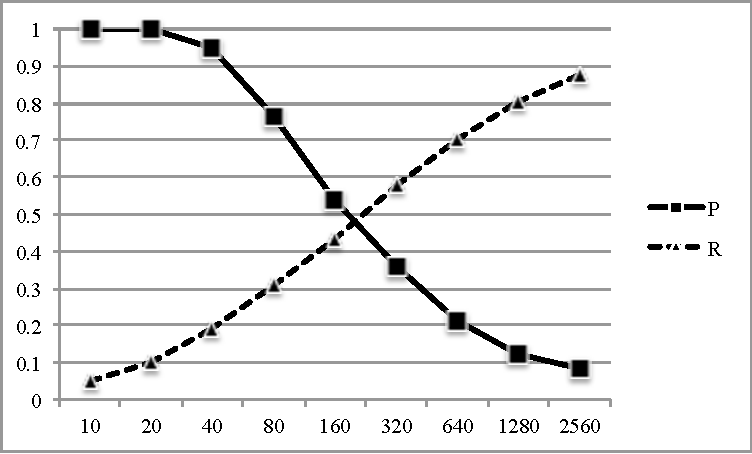
\includegraphics[width=240pt,height=160pt]{figures/ICAME_2013_27_BW.pdf}
\caption{Precision vs. recall curve of the light verb \expl{give} in the British National Corpus, using t-score \citep{ronan_schneider_mwe_15}.}
\label{discover-lightverbs}
\end{figure}


%\input{constantetal/05-joint}
\section{Joint approaches}
\label{sec:joint}

Joint approaches perform parsing and MWE identification simultaneously.
Since syntactic and lexical-semantic information are complementary, both processes can help each other if performed together.
In such systems, MWE lexical-seman\-tic segmentation is often seen as a by-product of syntactic analysis, or vice-versa.

Some MWEs require quite sophisticated syntactic information to be recognized, such as subcategorization frames and phrase structure.
Joint approaches favor delaying the decision as to whether a given combination is an MWE to the parser, where this information is available.
In other words, the system has access to the right information at the right moment. % in the pipeline.


Parser evaluation scores are often reported on standard test sets, where MWEs have been manually pre-identified (gold).
Jointly performing MWE identification and parsing is more realistic than parsing pre-annotated test sets, where MWEs are often represented as words with spaces (Figure~\ref{fig:wws}).
Indeed, when moving from standard test sets to real texts, gold MWE identification is not necessarily available.
It may be hard to use a pipeline approach (Sec.~\ref{sec:pipeline}) if the target MWEs are ambiguous or discontiguous.

On the downside, parsers that perform both syntactic analysis and MWE identification simultaneously are harder to design.
First, ambiguity is increased, often by a larger number of labels and/or parsing decisions that are possible at a given moment.
It is crucial, for such systems, to have coherent MWE annotations in treebanks, datasets that are large enough, and features that generalize well. 

We classify such approaches according to the degree of  ``MWE-awareness'' of the parser.
In shallow approaches, the parser generates $n$-best solutions without putting any particular emphasis on MWEs, then uses MWE information for reranking (Sec.~\ref{ssec:joint:rerank}).
The majority of joint approaches add MWE information to training and test treebanks, and then use off-the-shelf parsers enriched with dedicated MWE features (Sec.~ \ref{ssec:joint:data}). 
We also present fully MWE-aware parsers that take them into account in the parsing algorithm itself (Sec.~ \ref{ssec:joint:model}).


\subsection{N-best and reranking approaches }
\label{ssec:joint:rerank}

One possible orchestration solution is to consider MWE identification as a retokenization problem, as described in Subsection~\ref{ssec:concat}.
In $n$-best approaches, however, the text is first segmented into tokens in a non-deterministic way, considering \emph{several possible segmentations}.
Usually, the output of such non-deterministic tokenizer is a lattice containing all possible segmentation paths for a sentence \citep{sagot:2005}.
This representation is particularly suited for ambiguous irregular constructions, that could be considered as MWEs or as accidental co-occurrence, depending on the context.
The parser then must take this ambiguous segmentation and uses simple parsing models to disambiguate the input and generate a parse tree \citep{nasr:11}.

An $n$-best MWE identifier is used by \citet{constant13}, producing a lattice of possible segmentations. Then, a PCFG-LA parser is used to disambiguate the possible readings. The authors test two variants. First, they consider that MWEs in the lattice are single nodes (words with spaces). 
Thus, different segmentation possibilities in the lattice are represented by paths with different lengths. Second, they considering that MWE components are individual nodes tagged using an IOB scheme, like in Figure~\ref{fig:iob}. The latter obtains better performance because all possible paths in the lattice have the same length, resulting in more accurate parsing scores.

Conversely, the parser can use the same kind of approach and also generate $n$-best parsing trees.
A reranker can then use MWE-aware features, among others, to choose the highest scoring tree. \citet{constant12}, for instance, use a deterministic tokenizer but output $n$-best MWE-aware syntactic trees using the Berkeley constituent parser. Then, they use a discriminative reranker to choose the correct parse tree that includes MWE features.  




These are considered joint approaches because, even though MWE segmentation and parsing are independent processes, one needs to be aware of the format of the input/output of the other.
For example, the parser has to be able to process lattices as input, provided by the non-deterministic MWE identifier.





\subsection{Treebank modification approaches}
\label{ssec:joint:data}

In Section~\ref{sec:representation}, we discussed several ways to represent MWEs in treebanks.
Standard statistical parsers trained on such treebanks will be inherently aware of MWEs, provided that they can handle the particular MWE representation in that treebank.
For example, if MWEs are represented as subtrees (Figure~\ref{fig:extended-labels}), then there is no need to explicitly handle MWEs \citep{nivre16}.
This subsection covers MWE-aware parsing studies   in which the learning and parsing algorithms \emph{remain unchanged} with respect to their standard version.

Approaches discussed in this section face several challenges.
First, most of the time MWEs are either \main{absent} from treebanks, or the available representation requires \main{adaptations} in order to be usable by the parser.
Second, parsers learned from MWE-annotated treebanks often require \main{extra features} to take MWEs into account properly. Third, these features may suffer from data \main{sparseness}, as individual MWEs may not occur often enough in limited-size treebanks.\footnote{
Some MWE categories may never occur (\eg{} colloquial idioms) because many existing treebanks cover a single register (\eg{} newspapers).}

This subsection covers approaches that tackle the challenges that MWEs pose by:
\begin{itemize}
 \item adding or modifying the MWE representation in the treebanks, and/or
 \item adding MWE-dedicated features to the parsing model.
\end{itemize}
The last challenge, related to data sparseness and domain adaptation, is tackled by integrating external resources in the parser, as discussed in Section~\ref{sec:resources}.


In constituency parsing, several parsers, MWE representations and feature sets have been tested, especially on contiguous MWEs in the French Treebank. 
\citet{constant13} experiment with two implementations of a PCFG-LA parser, using a representation similar to the one of \citet{green11} and a variant similar to IOB encoding.

When MWE annotation is absent, a reasonably straightforward solution is to automatically project an MWE lexicon on the treebank before training the parser.
For instance, \citet{kato16.422} project a lexicon of compound function words (\eg{} \expl{a number of}) onto the English Ontonotes constituency treebank. 
Syntactic trees are modified to take MWEs into account.
Constituents are then automatically transformed into dependencies and a standard first-order graph-based parser is learned.
While the training data is modified, no MWE features are added to the model.

Early experiments on MWE-aware dependency parsing compared two representation variants: MWEs as subtrees or as words with spaces \citep{nivre04b}.
The results indicated that the subtree representation (joint approach) is worse than parsing MWEs as words with spaces (pipeline approach).
However, these results were obtained assuming gold MWE segmentation. %, which is not realistic.

\citet{vincze13} were among the first to use a dependency parser to perform realistic MWE identification.
They focus on light-verb constructions (LVCs) in Hungarian.
They first perform an automatic matching of two annotation layers in the Szeged Treebank: syntactic dependencies and LVCs.
As a result, the  dependency link between a light verb and a predicative noun (\eg{} {\scshape obj}) is suffixed with a {\scshape lvc} tag, whereas regular verb-argument links remain unchanged, like in Figure\ref{fig:extended-labels}. An off-the-shelf parser is used to predict the syntactic structure of sentences, including LVC links.
Given that Hungarian is a relatively free word-order language, LVCs often involve long-distance dependencies.
When compared with a classifier baseline, the parser performs slightly worse on contiguous LVC instances (F1=81\% vs. 82.8\%) but considerably better on discontiguous LVCs (F1=64\% vs. 60\%).


Treebanks containing MWEs as words with spaces pose problems when converted into subtrees. 
When splitting an MWE, one needs to manually or semi-automatically assign POS, lemmas and morphological features to the individual MWE components. 
Additionally, the internal syntactic structure must be inferred.
Since it is difficult to automate this task, the internal syntactic structure of decomposed MWEs is often underspecified using flat head-initial subtrees \citep{seddah13}, head-initial \citep{nivre16} or head-final chained subtrees \citep{eryigit:2011:mes:2206359.2206365}, as detailed in Section~\ref{ssec:subtrees}.
\citet{eryigit:2011:mes:2206359.2206365} compare parsing and MWE identification accuracy on different treebank representations for different MWE types.
Their original treebank includes MWEs as words with spaces, which are semi-automatically transformed into subtrees.
Contrary to previous conclusions \citep{nivre04b}, results indicate that subtrees may be a more suitable solution for some MWE types, specially when looking at MWE-aware parsing evaluation metrics (Sec.~\ref{sec:evaluation}). In this study, the words-with-spaces representation is shown to have a harming effect on the types, where it increases lexical sparsity, such as in Turkish light-verb constructions.

\citet{candito2014strategies} explore several orchestrations for combining syntactic parsing and contiguous MWE identification in French, distinguishing syntactically regular from irregular multiword constructions. In particular, they experimented with an off-the-shelf graph-based parser that was learned from an MWE-aware treebank where the subtrees representing regular and irregular expressions have their usual labels suffixed by the POS of the MWE, as shown in Figure~\ref{fig:extended-labels}. They showed on-par results with different pipeline variants.


\citet{nasretal15} focus on ambiguous compound grammatical words in French of the form ADV+\expl{que} and \expl{de}+DET.
While these represent a limited scope, such constructions are pervasive and hard to identify without access to syntactic information, because its component words can co-occur by chance. %, making it hard to disambiguate them.
For instance, the two sentences below have the same sequences of POS and similar lexical units, but the first one contains an MWE whereas the second one does not:

\ea
\gll Je chante {\textbf{bien}} {\textbf{que}}  je sois triste\\  
     I  sing   well       that       I  am   sad\\
\glt `I sing even though I am sad'
\z 

\ea
\gll Je pense {\textbf{bien}} {\textbf{que}}  je suis triste\\  
     I  think well       that       I  am   sad\\
\glt `Indeed, I think that I am sad'
\z

In order to deal with these constructions, the training treebank is modified similarly to \citet{candito2014strategies}, splitting MWEs originally represented as words with spaces into two tokens linked by a special dependency. 
For example, since \expl{bien que} functions as a conjunction, the conjunction \expl{que} becomes the head, modified by the adverb \expl{bien}. % using a {\scshape Morph} link.
Using a standard graph-based dependency parser, the authors evaluate the identification of the target MWEs on a dedicated dataset. As described in Section~\ref{ssec:lex-help-mwe}, the use of subcategorization frame information for verbs, coming from an external lexicon, improves the results.


\subsection{MWE-aware parsing models}
\label{ssec:joint:model}

The models discussed up to now have the advantage of being simple and fast to deploy.
Provided that the training treebank contains MWEs in a suitable representation (which can be manually or automatically converted), the parsing algorithm itself does not need to be changed to accommodate MWEs.
These approaches achieve reasonably good results, specially if compared to MWE systems based on purely sequential models.
However, they often use language-specific or treebank-specific workarounds and are not always generalizable.
Therefore, some recent contributions focus on designing parsing models that are truly awa\-re of MWEs in the model, with promising results.

In the framework of constituency parsing, \citet{green11} propose and evaluate an MWE-aware parser based on tree substitution grammars (TSGs).
This work was latter extended, comparing the TSG with a PCFG model enriched with a factorized lexicon \citep{green13}.
The authors apply these models to MWE-rich treebanks for French and Arabic, showing gains for both parsing and MWE identification.
The authors state that TSGs are more powerful than PCFGs, being able to store lexicalized tree fragments.
They are therefore more suitable for idiomatic MWEs, whose particular syntactic analysis requires larger contexts to be predicted.

Along the same lines, \citet{leroux14} design a joint parsing and MWE identification model based on dual decomposition.
In this work, however, a specialized sequence model performs lexical segmentation of MWEs.
The MWE identification module uses conditional random fields, while the parsing module uses a PCFG-LA also including MWE identification, using the approach of \citet{green13}. 
Both models are combined using penalty vectors that are updated in an iterative way.
In other words, until reaching consensus on MWE identification, the MWE identifier and parser analyze the input sentence.
If the systems do not agree, they are penalized in proportion to the difference between the given solution and the average solution.
This model reaches impressive performance on the French treebank, reaching an MWE identification F-score of up to 82.4\% on the test set.


\citet{constantnivre16} propose a new dependency parsing system that jointly performs syntactic analysis and lexical segmentation (including MWE identification).
The authors design and evaluate a transition-based parser using two synchronized stacks: one for syntactic parsing and another for lexical segmentation.
The synchronization of both stacks is guaranteed by a unique {\scshape Push} transition which pushes the first element of the buffer on both stacks.
The parser models MWE-dedicated transitions {\scshape Merge$_N$} and {\scshape Merge$_F$}, which respectively create new merged lexical nodes for regular MWEs and lexico-syntactic nodes for fixed MWEs.
An additional {\scshape Complete} transition marks that a given lexical node has been fully parsed (but can be implicit). This approach obtains results that compare with or exceed state-of-the-art performance on French and English MWE-rich treebanks.
Finally, the authors show that lexical information can guide parsing, leading to slightly better syntactic trees.
The converse assumption does not seem to hold, though, as adding syntactic information to a purely lexical parser tends to slightly degrade its performance.



%\input{constantetal/06-resources}
\section{Integration of lexical resources}
\label{sec:resources}

Lexical resources are large-scale repositories of information typically about simple words, more rarely about MWEs. 
They can play different roles with respect to statistical MWE-aware parsing, and in this section we discuss three of them. We show how lexical information can help in general to resolve parsing ambiguities (Sec.~\ref{ssec:lexres-parse}). Then, we focus on the availability of lexical information within pipeline approaches (Sec.~\ref{ssec:mwe-help-parse}). Finally, we shift the emphasis to the effect of lexical resources on MWE identification rather than on parsing itself (Sec.~\ref{ssec:lex-help-mwe}).

\subsection{General integration of lexical resources in statistical parsers}
\label{ssec:lexres-parse}

Statistical parsers have several drawbacks due to the limited size of available gold standard treebanks used for training. Many words in the datasets are  infrequent, which makes it very difficult to learn relevant (lexical) regularities. In addition, when parsing an unseen text, some words are simply absent from  the training dataset, which negatively impacts parsing accuracy. Experiments with  different solutions have been undertaken within the parsing community, notably by incorporating external resources mostly (but not only) learned automatically from large raw corpora.

The use of word clusters is one method to deal with the lexical sparsity issue. Clusters (\eg{} Brown clusters), consist of groups of words occurring in the same  context. 
Replacing words by clusters or using clusters as features has each been shown to improve parsing accuracy  \citep{koo-carreras-collins:2008:aclmain,candito-seddah:2010:spmrl}.
Pairs of words that co-occur frequently in large corpora tend to be related syntactically. 
The provision of information about such lexical affinities to the parser has been shown to usefully support  syntactic attachment decisions. 
Lexical affinities might be integrated using either soft constraints \citep{bansal:11,mirroshandel:12} or hard ones \citep{mirroshandel:2016}. 
The deep learning revolution has opened new perspectives to help handle lexical sparsity, as words are represented as continuous space vectors (\ie{} word embeddings) learned from large corpora. Words having similar syntactic behaviors have vectors that are geometrically close to each other \citep{durrett:15,dyer:15}.

The use of external lexicons has also turned out to be of great interest, notably for dependency parsing. For instance, \citet{candito:2010} successfully use the MELt tagger \citep{denis:2012}, thereby incorporating features based on a large-scale morphological lexicon. The integration of hard constraints based on syntactic lexicons was also shown to have a positive impact \citep{mirroshandel:2013}. 


\subsection{MWE resources help parsing}
\label{ssec:mwe-help-parse}

We now give examples of MWE lexical resource integration using a pipeline approach (Sec.~\ref{sec:pipeline}) in which MWEs are replaced by their syntactic heads. We do so on two levels: general NP chunking and technical terms.


On the chunking level, replacing chunks with their head words reduces parsing complexity considerably. 
According to experiments carried out by \citet{prins05}, parsing performance also increases slightly. 
However, experiments on technical terms have not confirmed this hypothesis.
In other words, replacing chunks with their heads does not necessarily lead to improved results in other settings. 


\citet{weeds-ea07} used a substitution approach (Sec.~\ref{ssec:subst}) for term identification in the domain of biomedical research, where gene and protein names in particular are often MWEs. Because taggers, unless they are trained on the domain, perform very poorly, they report better results when replacing technical terms with their head, using a large lexicon of domain terms.\footnote{Such a lexicon is often referred to as \emph{gazetteer}.}

A comparable example is the situation in which a sentence such as 
%
\expl{... he did not see the traffic\_N light\_V} 
%
is POS-tagged incorrectly (\expl{light\_V instead of light\_N}). Here, a pipeline substitution approach relying on an MWE lexicon can clearly improve results. This improvement is passed on to the subsequent parsing step. 
When domain-adapted taggers are available, though, the advantages of the substitution approach tend to disappear. 
The performance of adapted taggers is often comparable or slightly higher than that of the substitution approach, as tagging accuracy of technical terms increases. 
In short, sometimes it is better to adapt statistical models (in this case, a domain-adapted tagger) rather than using lexical resources (in this case, an MWE gazetteer of the domain).% 

\citet{schneider:2014} conducted an experiment using LT-TTT2, an off-the-shelf rule-based named entity recognizer \citep{grover08} on the standard evaluation suite GREVAL \citep{carroll-ea04} with the same approach of replacing multiword named entities by the head of the MWE. The performance of the substitution approach was slightly worse than when leaving the MWE unchanged. %\todo{CR: worse than what? => I told you I'm picky :-P} 
Also this experiment did confirm that statistically motivated resources are usually better than purely lexical resources.


\subsection{Lexical resources help MWE-aware parsing}
\label{ssec:lex-help-mwe}

Having discussed the effect of lexical resources on parsing accuracy, we now turn to two different ways to use them as a source of features for dependency parsers, to help MWE identification as well as parsing accuracy. 

The first is to use MWE lexicons to alleviate the low coverage of MWEs in the training dataset. The idea is to perform an MWE pre-segmentation of the input text by lexicon lookup. The pre-segmentation, encoded in an IOB-like format, is then used as source of features during MWE-aware parsing, either in the parser itself for joint approaches \citep{candito2014strategies}, or in the MWE tagger applied before parsing in pipeline approaches \citep{constant12,constant:13:mwe}.  

One advantage of using soft constraints like features is their ability to handle ambiguous MWEs.
Let us take the sequence \expl{up to}, which can be either a complex preposition (\expl{no more than}) or an accidental co-occurrence (\expl{look up to the sky}). A naive segmentation will systematically consider it to be an MWE, independently of the context. However, a better decision can be made taking the context (\ie{} the set of other features) into account. Using a joint approach on the French treebank, \citet{candito2014strategies} managed to gain around 4 points in terms of tagged MWE identification F-score using such lexicon-based features: F1=74.5 (with) vs. F1=70.7 (without). We should recall, however, that their approach is limited to contiguous MWEs.


A second method proposed by \citet{nasretal15} is to incorporate subcategorization frame information, derived from a syntactic lexicon, as features in a joint parser. This was used to improve the resolution of ambiguities between grammatical compound MWEs and accidental co-occurrences.
An example is the French sequence \expl{bien que} which is either a multiword conjunction (\expl{although}) or  an adverb (\expl{well}) followed by a relative conjunction (\expl{that}), as exemplified in Subsection~\ref{ssec:joint:data}. This ambiguity may be resolved using information about the verb in the syntactic neighborhood. The authors included specific features indicating whether a given verb accepts a given complement: \expl{manger (to eat)} -QUE -DE, \expl{penser (to think)} +QUE -DE, \expl{boire (to drink)} -QUE -DE, \expl{parler (to speak)} -QUE +DE. 
In particular, they show for French that there is a 1-point gain in F-score, 85.24 (without) vs. 86.41 (with), for MWEs of the form ADV+\expl{que} (ADV+\expl{that}). The effect is spectacular for compounds of the form \expl{de}+DET, that display a 15-point gain : 75.00 (with) vs. 84.67 (without).

  

%\input{constantetal/07-evaluation}
\section{Evaluation}
\label{sec:evaluation}



Evaluating a syntactic parser generally consists in comparing the output to reference  (gold-standard) parses from  a manually labeled treebank.
In the case of constituency parsing, a constituent is treated as correct if there exists a constituent in the gold standard parse with the same labels, starting and ending points. These parsers are traditionally evaluated through precision, recall and F-score \citep{abney1991procedure,sekine1997evalb}. 

In standard dependency parsing with single-head constraint\footnote{Each dependent node has at most one head in the produced dependency tree.}, the number of dependencies produced by a parser is equal to the number of total dependencies in the gold-standard parse tree. Common metrics to evaluate these parsers include the percentage of tokens with correct head, called \emph{unlabelled attachment score} (\asu), and the percentage of tokens with correct head \emph{and} dependency label, called labeled attachment score (\asl) \citep{conllx,nilsson2007conll}. 

The evaluation of MWE-aware parsers and the evaluation of  whether or not MWE pre-identification helps  improving the parsing quality should be carefully carried out.
As stated in previous sections, in most works where MWE identification is realized before parsing, the MWEs are merged into  single tokens.  
As a result, the common metrics for parsing evaluation given above become problematic for measuring the impact of MWE identification on parsing performance \citep{eryigit:2011:mes:2206359.2206365}.
For example, in dependency parsing,
the concatenation of MWEs into single units  decrements the total number of evaluated dependencies. It is thus possible to obtain different scores without actually changing the quality of the parser, but simply the representation of the results. Instead of \asu~ and \asl~ metrics, the attachment scores on the surrounding structures, namely \asus~ and \asls~ (\ie{} the accuracy on the dependency relations excluding the ones between MWE elements) are more appropriate for extrinsic evaluation of the impact of MWE identification on parsing. Similar considerations apply to constituency parsing.

\begin{figure*}[htbp]
  \centering
%  \begin{turn}{-.8}
      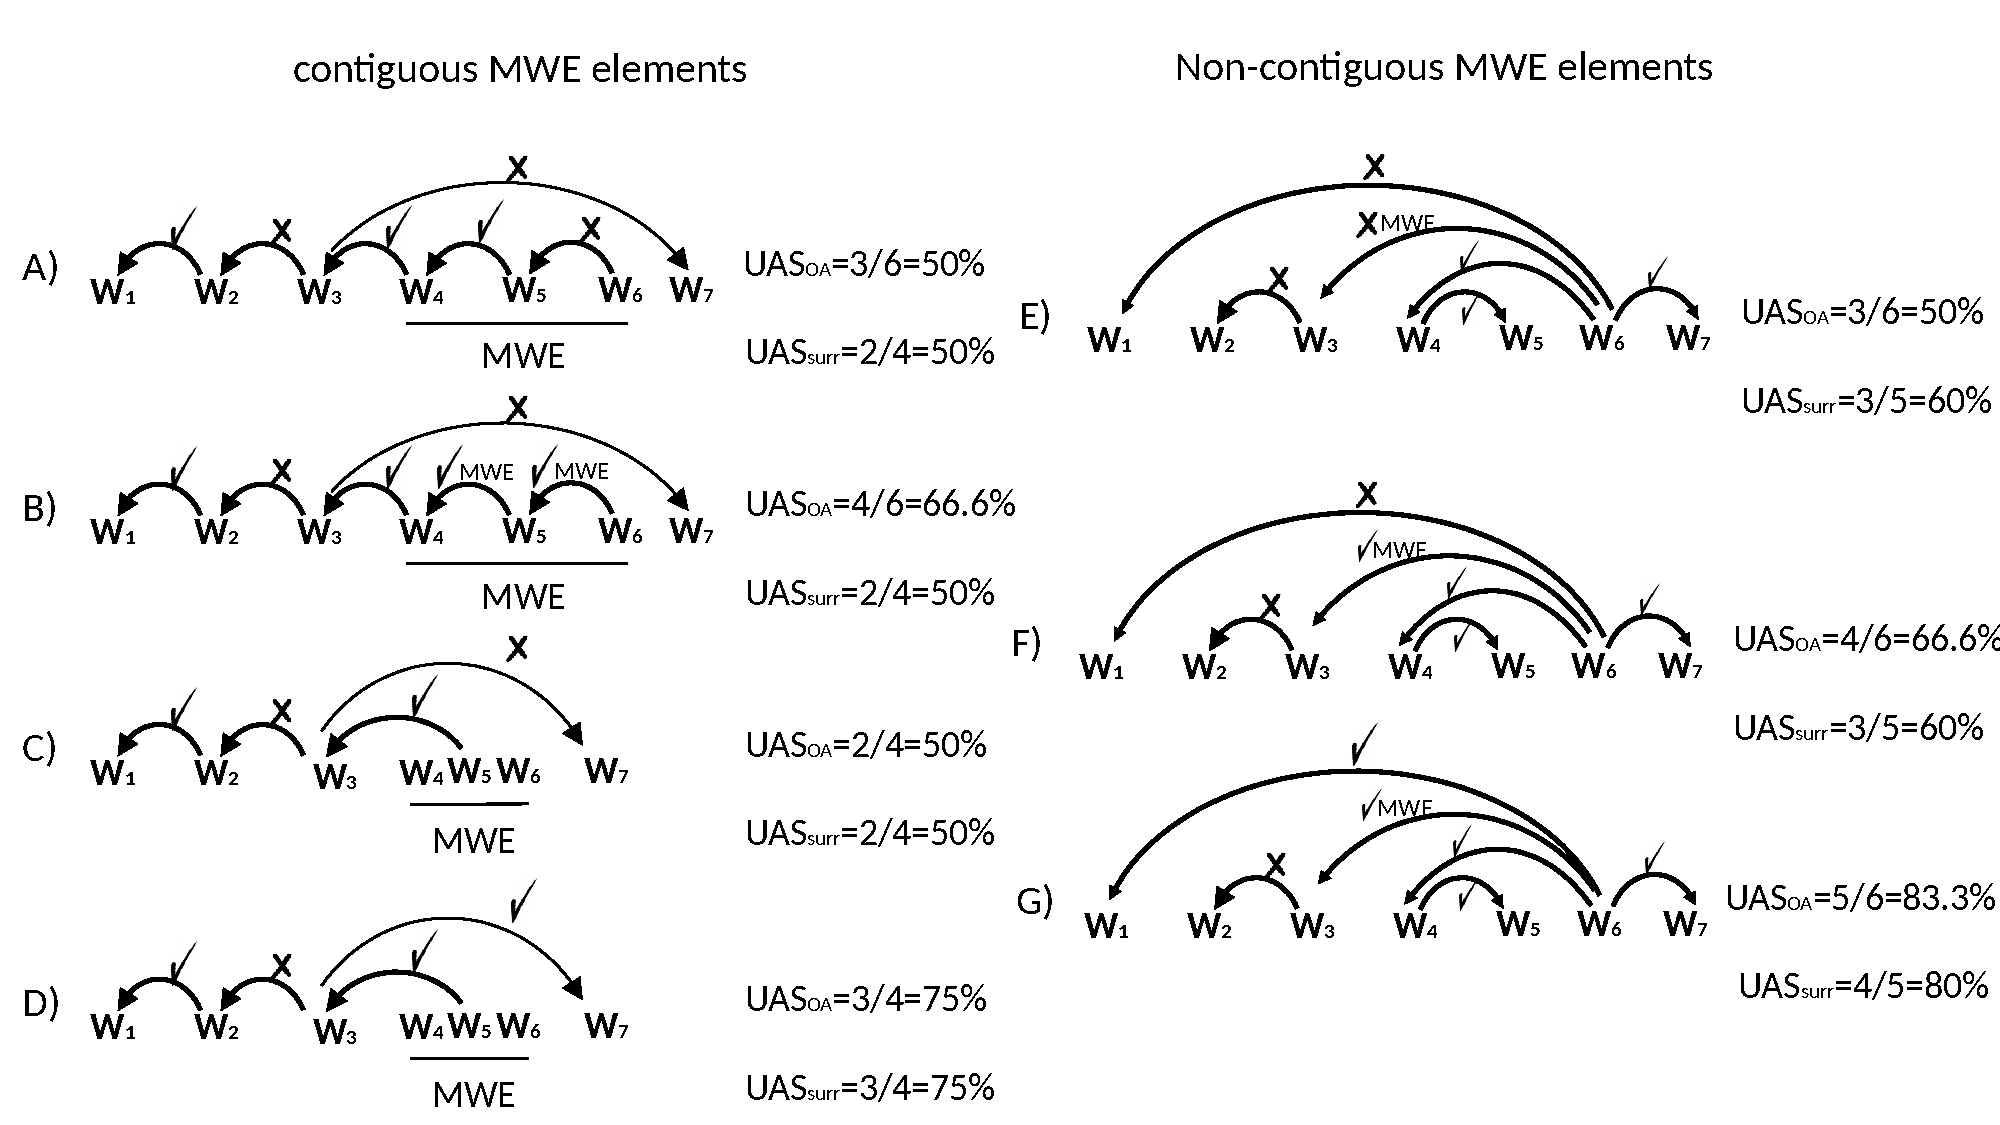
\includegraphics[width=1.00\textwidth]{figures/Presentation1}%example-constant.png}
%    \end{turn}
    \caption{Extrinsic evaluation examples of the impact of MWE identification on dependency parsing performances.}
	\label{fig:example}
\end{figure*}


Figure~\ref{fig:example} provides two example sequences for the phenomena discussed above; one containing a contiguous MWE (on the left side)  and another one containing a non-contiguous MWE (on the right side).
The dependency trees in this figure provide the gold standard unlabeled dependency relations for both examples.
Correctly predicted dependencies %by the used setting 
are presented with check marks (\checkmark) over the relations, whereas the wrongly predicted dependencies are presented with a cross mark (\ding{55}). 
The contiguous MWE of the left side sequence consists of three tokens (w$_4$, w$_5$ and w$_6$). In other words, the two dependency relations of the overall sequence belong to the relations between MWE elements. The non-contiguous MWE of the right side sequence consists of two tokens (w$_3$ and w$_6$).

The first examples of each column (``(A)'' and ``(E)'') show the success of a dependency parser without any prior MWE identification process. 
In the remaining settings, an MWE identifier is run over the given sequence before parsing.
Both the overall unlabeled accuracy \asuo{} and the accuracy of the surrounding structures \asus{} are provided next to the trees. Examples ``(B)'', ``(C)'' and ``(D)'' show the correctly detected relations by applying an MWE identifier prior to the syntactic parsing. In ``(C)'' and ``(D)'', the detected MWE is combined into a single unit (w$_4$w$_5$w$_6$) whereas in ``(B)'', the detected MWE is represented as a subtree. % constraint to the syntactic parsing.

%One may notice from this example that i
In ``(A)'', ``(B)'' and ``(C)'', although the parser success does not change on detecting the syntactic dependencies, \asuo~ is affected by the total number of evaluated dependencies, whereas \asus~ remains stable, as expected.
In ``(D)'', MWE identification helps the parser to detect one more dependency relation which, is reflected in \asus{}.
Similarly, in ``(F)'', the pre-identification of  ``w$_3$ - w$_6$'' MWE has no impact on the parser's performance.
%\mycyan{
Although this can be directly observed by \asus~(60\%), \asuo~ mistakenly gives the impression of an improvement in parsing performance (50\%$\Rightarrow$66.6\%). This is because  in this setting (second column of Figure~\ref{fig:example})
%2nd column non-contiguous MWE elements), 
\asuo~ evaluates the performance of MWE pre-identification and dependency parsing as a whole.
%}
In ``(G)'', the parser performs better after MWE identification, which is again reflected in the surrounding structure evaluation.

Although \asus~ and \asls~ are valuable scores for measuring the impact of identifying different MWE types on parsing performance, they are troublesome with automatic MWE identification, when gold-standard MWE segmentation is not available. Then, erroneous MWE identification would degrade parsing scores on the surrounding dependencies.
An alternative solution is to detach the concatenated MWE components (if any) into a dependency or constituency subtree \citep{candito2014strategies,eryigit:2011:mes:2206359.2206365}. This way, the standard evaluation scores \asu{} and \asl{} are still applicable in all different orchestration scenarios, for both contiguous and non-contiguous MWEs, successfully assessing the performance of joint syntactic parsing and MWE identification as a whole.

%\input{constantetal/08-conclusions}
\section{Conclusions}
\label{sec:conclusions}


In this chapter, we 
elaborated upon
several approaches for combining MWE processing with statistical parsing to yield statistical MWE-aware parsing. These approaches depend on different parameters such as MWE representation, orchestration and external resource integration. First of all, the selected MWE representation combined with syntactic analysis have a strong impact on the system implementation, since 
the more elaborated and hence more linguistically expressive the representation is, the more complex the computational system has to be.
Representations vary from simple words with spaces to multilayer structures. The timing of MWE identification with respect to syntactic parsing, namely orchestration, is a crucial feature that needs to be carefully taken into account when designing a statistical MWE-aware parser, as the best choice partly depends on MWE type under consideration. MWE identification may be performed before, after, or during parsing. The first two were discussed under the rubric ``pipeline'' approaches in Section~\ref{sec:pipeline}; the third, under ``joint'' approaches, in Section~\ref{sec:joint}. Last, we showed that the use of external resources is another important feature that is required to handle the sparsity problem, not only to support syntactic attachment decisions, but also MWE identification. 

Although it is difficult to draw hard and fast conclusions, it seems that further investigation of dedicated MWE-aware parsing models is 
called for.
Such models can benefit from joint modeling of closely related tasks, with information from one layer helping to disambiguate the other. 
Joint approaches seem to offer a very promising line of research, as has been shown for other NLP tasks: \eg{} joint POS tagging and parsing \citep{bohnet:2013}, joint syntactic and semantic parsing \citep{henderson:2013}. Such approaches are now becoming prominent in NLP alongside the deep learning revolution. In fact, most joint approaches to statistical MWE-aware parsing are not truly joint, as they consist of workaround solutions. We saw how many studies investigated the use of off-the-shelf parsers by modifying training data, thus making the datasets MWE-aware. Truly joint systems are rarer, requiring the use of specific grammatical formalisms for constituency parsing or the development of new dependency parsing mechanisms dedicated to MWE identification. 

As a consequence, there is much ground for future work.
However, special emphasis should be given to the development of MWE-rich treebanks.
Not only are these resources lacking for many languages, but also the representation and covered MWE types vary considerably among different resources.
We believe that the development of new MWE-aware parsing models and resources would enable satisfactory solutions for this hard problem.
Such solutions could then be further integrated into downstream applications, taking a significant step towards semantic processing of MWEs, and thus of a key element of language itself.


\section*{Acknowledgements}

This work was supported by the PARSEME action (COST IC1207).  It was also partially funded by the French National Research Agency (ANR) through the PARSEME-FR project (ANR-14-CERA-0001) and by a TUBITAK 1001 grant (no: 112E276).
%We are thankful to XXX

\printbibliography[heading=subbibliography,notkeyword=this]

\end{document}
